\documentclass[letterpaper,12pt]{article}
\usepackage{tabularx} % extra features for tabular environment
\usepackage{amsmath}  % improve maths presentation
\usepackage{amssymb} % maths symbols
\usepackage{graphicx} % takes care of graphic including machinery
\usepackage[margin=0.95in,letterpaper]{geometry} % decreases margins
\usepackage{cite} % takes care of citations
\usepackage[titletoc,title]{appendix} % takes care of appendices
\usepackage{listings} % code representation
\usepackage{pdflscape}
\usepackage{csquotes} % for quoting existing work
\usepackage{color} % defines colours for code listings
\usepackage{comment} % allows for block of comments
\usepackage{gensymb} % degree symbol
\usepackage[table,xcdraw]{xcolor} % table colouring
\usepackage[cc]{titlepic}  % allows a pic to be included in the title page
\usepackage[final]{hyperref} % adds hyper links inside the generated pdf file
\usepackage{pdfpages} % include pdfs

% style code listings
\definecolor{codegreen}{rgb}{0,0.6,0}
\definecolor{codegray}{rgb}{0.5,0.5,0.5}
\definecolor{backcolour}{rgb}{0.95,0.95,0.92}
\lstdefinestyle{mystyle}{
    backgroundcolor=\color{backcolour},   
    commentstyle=\color{codegreen},
    keywordstyle=\color{blue},
    numberstyle=\tiny\color{codegray},
    basicstyle=\footnotesize,
    breakatwhitespace=false,         
    breaklines=true,                 
    captionpos=b,                    
    keepspaces=true,                 
    numbersep=5pt,                  
    showspaces=false,                
    showstringspaces=false,
    showtabs=false,                  
    tabsize=4
}
\lstset{style=mystyle}

\begin{document}

\title{
    CS5011 Artificial Intelligence Practice\\Assignment 4 Report\\
    \begin{large}
    University of St Andrews - School of Computer Science
    \end{large}
}
\titlepic{
\includegraphics[width=0.3\linewidth]{report/figures/st-andrews-logo.jpeg}}
\author{Student ID: 150014151}
\date{20th December, 2019}
\maketitle
\newpage

\tableofcontents
\newpage


% --------------------------------------- 1 - INTRODUCTION ------------------------------------------ 

\section{Introduction}
\label{sec:introduction}

The following requirements were attempted:
\begin{itemize}
    \item Basic Agent:
    \begin{itemize}
        \item Multilayer feedforward neural network.
        \item Data encoding and training/testing split.
        \item Training/testing result visualisation in plots and heatmaps.
        \item Grid search algorithm for determining optimal hyperparameters.
    \end{itemize}
    \item Intermediate Agent:
    \begin{itemize}
        \item CLI text-based interface.
        \item Early predictions.
        \item Neural network re-training.
    \end{itemize}
        
\end{itemize}

\subsection{Installation}

Create a virtual environment for the project and activate it:

\begin{lstlisting}
virtualenv ~/Environments/A4
source ~/Environments/A4/bin/activate
\end{lstlisting}

Once you have the virtual environment activated, \textit{cd} into the project directory and install the requirements needed to run the app:

\begin{lstlisting}
pip install -r requirements.txt
\end{lstlisting}

\subsection{Usage}

To compile the program, navigate to the \textit{A4src} directory and run the following command:

\begin{lstlisting}
python A4Main.py [-h] -a <AGENT> -c <CSV> [-g] [-d]
\end{lstlisting}

where:

\begin{itemize}
    \item \textit{AGENT} is the type of agent to run: \textit{[Bas, Int, Adv]}:
    \begin{itemize}
        \item \textit{Bas}: Train and test the neural network with the optimal parameters, or run the Grid Search algorithm to determine the optimal parameters.
        \item \textit{Int}: CLI text-based application to submit a new ticket and predict to which response team it should go.
        \item \textit{Adv}: todo.
    \end{itemize}
    \item \textit{CSV} is the CSV file containing the data used to train/test the data.
    \item \textit{-g}: is a flag that run the grid search algorithm when set.
    \item \textit{-d}: is a flag that enters \textit{debugging} mode, printing more statements to the command line, when set.
    \item \textit{-h}: is a flag for printing help on how to use the program.
\end{itemize}

\paragraph{Examples}

Here are a few examples that can be used to run the program:

\begin{itemize}
    \item ``\textit{python A4Main.py -a Bas -c tickets -d}'' to train/test the neural network.
    \item ``\textit{python A4Main.py -a Bas -c tickets -g}'' to run the grid search algorithm.
    \item ``\textit{python A4Main.py -a Int -c tickets}'' to submit a new ticket through the CLI text-based interface
    \item ``\textit{python A4Main.py -h}'' for help on how to run the agent.
\end{itemize}

\subsection{Tools Used}

\begin{itemize}
    \item Scikit\footnote{Scikit: \url{https://scikit-learn.org}} and related Python libraries (e.g. NumPy\footnote{NumPy: \url{https://numpy.org/}}, Pandas\footnote{Pandas: \url{https://pandas.pydata.org/}}, Matplotlib\footnote{Matplotlib: \url{https://matplotlib.org/}}).
    \item PyCharm\footnote{PyCharm: \url{https://www.jetbrains.com/pycharm/}}: an IDE developed by JetBrains to write Python code with support for some of the above libraries.
    \item Git and GitHub: to back and version control the code.
    \item PEP8\footnote{PEP8: \url{https://www.python.org/dev/peps/pep-0008/}} coding guidelines and docstring followed throughout the entire code.
\end{itemize}

% -------------------------- 2 - DESIGN - IMPLEMENTATION - EVALUATION -------------------------------

\clearpage
\section{Design, Implementation \& Evaluation}
\label{sec:design-implementation-evaluation}

\subsection{Design: PEAS Model}

This section defines the PEAS model for a ticketing routing-based agent that uses a multilayer feedforward neural network in order to learn how to predict the appropriate response team for future tickets.

\paragraph{Performance measure}\label{sec:performance-measures} The basic agent's training efficiency can be evaluated with the error loss curve, and the testing accuracy by using a confusion matrix. The intermediate agent can be assessed by the correctness of its predictions.

\paragraph{Environment} This is a single-agent and fully-observable environment represented by a neural network and the text-based interface used to interact with a user logging a new ticket. Additionally, it can be said that the basic agent environment is deterministic (the next state is determined by the current state and the action executed) and stochastic for the intermediate agent (user input is unknown), according to the definitions set by Russell \& Norvig in \textit{Artificial intelligence: a modern approach} \cite{russell2016artificial}.

\paragraph{Actuators} The agent may accept input and target data it can learn from by backpropagating the calculated error between the input and target data in order to adjust the weights of the neural network (Stochastic Gradient Descent). It may also predict an output based on unseen data.

\paragraph{Sensors} The basic agent is always aware of the environment and can calculate feedback error based on input and target data, while the intermediate agent can receive responses to questions by interacting with a human user.

% ----------------------------------

\subsection{Implementation}

\subsubsection{Project Structure}

The project is divided in three main sections:

\begin{itemize}
    \item The \textit{agents} module, containing functions to implement the execution of flow of each agent.
    \item The \textit{neural\_network} module, which contains classes to create and manipulate a multilayered perceptron, a data encoder/processor and the grid search algorithm.
    \item The \textit{main} section, containing the program's entry point \textit{A4Main.py} for parsing the command line arguments, global configuration settings in \textit{config.py} and printing methods in \textit{helpers.py}.
\end{itemize}

The \textit{data} directory stores the CSV data, the \textit{neural\_networks} directory the trained neural nets in \textit{``*.joblib''} format, and the \textit{results} directory the various output of the agents. See Appendix \ref{sec:appendix-project-file-structure} for the full project structure.

% ----------------------------------

\subsubsection{Neural Network Training \& Testing (Basic Agent)}
\label{sec:basic-agent}

The basic agent takes a CSV file as input to be used for training and testing. It instantiates the custom \textit{DataProcessor} class containing functions for parsing the CSV file (retrieving tags and categories) and splitting the data between inputs and targets before encoding/decoding it. When being passed around, the data is often held in a \textit{DataFrame}\footnote{Pandas DataFrame: \url{https://pandas.pydata.org/pandas-docs/stable/reference/api/pandas.DataFrame.html}}, which allows for more manipulation than Python's built-in \textit{list}. The input data is encoded in either 0s or 1s, while the target data is encoded using one-hot encoding. Figure \ref{fig:data_encoding} depicts how the data is split and encoded.

\begin{figure}[h] 
\centerline{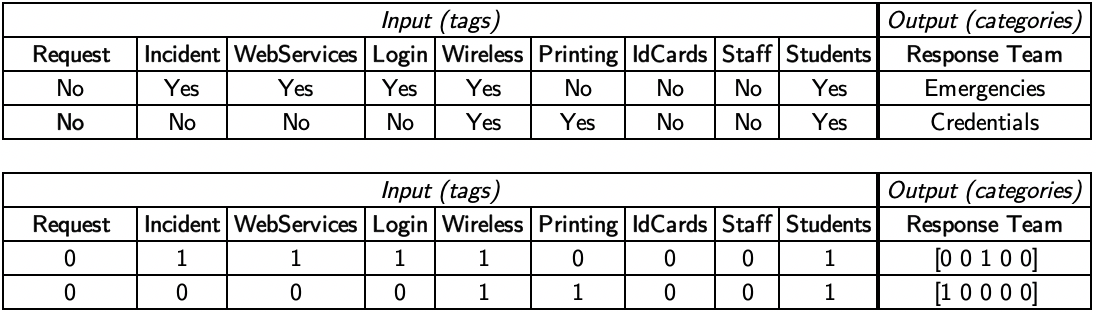
\includegraphics[width=\textwidth]{report/figures/data_encoding.png}}
\caption{\label{fig:data_encoding}Encoding of the data. At the top, the decoded data; at the bottom, the encoded data.}
\end{figure}

The data must be fed to the neural network in binary form. One-hot encoding is therefore chosen as it suits the sparse representation of the data, which is made up of only five target categories. Only a single digit may have the value 1 in one-hot encoding, while the others remain at value 0 \cite{lec16}. The one-hot encodings of the target categories can be seen in Figure \ref{fig:one_hot_encoding}.

\begin{figure}[h] 
\centerline{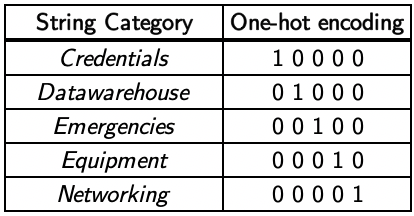
\includegraphics[width=0.4\textwidth]{report/figures/one_hot_encoding.png}}
\caption{\label{fig:one_hot_encoding}One-hot encoding of the categories.}
\end{figure}

Once the data is encoded, an instance of the custom \textit{MultiLayerPerceptron} class is created, containing functions to split the training/testing data, training \& testing the neural network, displaying results and saving the network with the trained weights. This custom class allows it to be easily re-used in the intermediate agent, thus avoiding code duplication. The class uses \textit{Scikit}'s \textit{MLPClassifier}\footnote{Scikit MLPClassifier: \url{https://scikit-learn.org/stable/modules/generated/sklearn.neural_network.MLPClassifier.html}} to implement the neural network and is instantiated with the optimal hyperparameters determined in Section \ref{sec:optimal-hyperparams}, which can be overwritten when creating a new \textit{MultiLayerPerceptron} (see Listing below).

\begin{lstlisting}[language=Python]
class MultiLayerPerceptron:
    def __init__(self, name, input_data, target_data, hidden_layers_size=(15,), solver="adam", activation_function="logistic", learning_rate_init=0.6, momentum=0.9, optimisation_tolerance=0.0001, num_iterations_no_change=1000, max_iterations=10000, verbose=config.debug):
\end{lstlisting}

An 80\%/20\% split is used for the training/testing data sets, with equal category distribution maintained between the training and testings sets, which is ensured through the use of the \textit{stratify} option in Scikit's \textit{train\_test\_split} function\footnote{Scikit train\_test\_split: \url{https://scikit-learn.org/stable/modules/generated/sklearn.model_selection.train_test_split.html}}. Because the data has 250 even entries (50 for each of the five outputs), the testing set will therefore have 10 entries for each of the five categories\footnote{250 data entries, 50 per response team, 80\%/20\% data split so 10 of each end up in the training set.}.\\

The actual training is carried out using the \textit{fit} function, with the \textit{error\_loss\_} plotted with regards to the number of epochs; while the testing is performed using the \textit{predict} and \textit{predict\_proba} functions and its accuracy visualised with a confusion matrix (counting the number of true positives/negatives and false positives/negatives) in a heatmap. These results can be visualised in Section \ref{sec:eval-errorloss-cm}.

% ----------------------------------

\subsubsection{CLI-Based Ticketing-Routing Agent (Intermediate Agent)}

The intermediate agent is built on a CLI\footnote{Command Line Interface} as an interactive text-based application allowing a human user to submit a new ticket. The agent records the \textit{``Yes''}/\textit{``No''} answers to each tag to create a new ticket, which is then used as input for the previously trained neural network to make a prediction. The neural net is loaded using \textit{joblib} and tested using the \textit{predict} and \textit{predict\_proba} function.\\

To avoid the repetitive task of answering all questions, the agent makes early predictions after the third, fifth and seventh questions. The prediction is made by filling out the missing fields in the ticket with the most common value (\textit{mode}) in the original CSV data.\\

After an early prediction is made, the user can state whether he is happy with the result or not. If he is not, the agent asks more questions until the next early prediction or until all questions have been answered. Finally, if the user is not happy with the final prediction, he can specify the desired response team to send the ticket to (only if he has answered all questions and entered \textit{``No''} to every early prediction). This information is added to the end of a copy of the original CSV data file that is used to re-train the neural network in a similar fashion mentioned in Section \ref{sec:basic-agent}. The newly trained network is then saved and used for future predictions.

% ----------------------------------

\subsubsection{Advanced}

todo


% ----------------------------------

\subsection{Evaluation}
\label{sec:evaluation}

\subsubsection{Optimal Hyperparameters}
\label{sec:optimal-hyperparams}

In order to find the optimal hyperparameters to train the neural network, a grid search algorithm is implemented. The algorithm exhaustively trains and tests the neural network with every combination from a pre-defined set of parameters and measures its accuracy. The parameters tested include the number of neurons in the hidden layer, the solver, the activation function, the learning rate, the momentum, the tolerance and the maximum number of iterations after which training stops if error does not improve by the tolerance. These can be found in the Listing below:

\begin{lstlisting}[language=Python]
grid_search_params = {
    `hidden_layer_sizes': [(3,), (5,), (7,), (9,), (15,), (25,)],
    `solver': ["sgd", "adam"],
    `activation': ["logistic", "relu", "tanh"],
    `learning_rate_init': [0.05, 0.1, 0.2, 0.4, 0.6, 0.8, 1.0],
    `momentum': [0.1, 0.3, 0.5, 0.7, 0.9],
    `tol': [1, 0.1, 0.01, 0.001, 0.0001],
    `n_iter_no_change': [100, 1000],
    `max_iter': [10000]  # Parameter not being tested.
}
\end{lstlisting}

Overall, 12,600 unique combinations of parameters were tested in 1h26m. From these tests, 14 combinations of hyperparameters with a +98\% mean accuracy (over 5 runs for even 80\%/20\% data splits) emerged as optimal, as depicted in Figure \ref{fig:gridsearch_results}. These optimal parameters can be found in more detail in Appendix \ref{sec:appendix-optimal-hyperparameters}.

\begin{figure}[h] 
\centerline{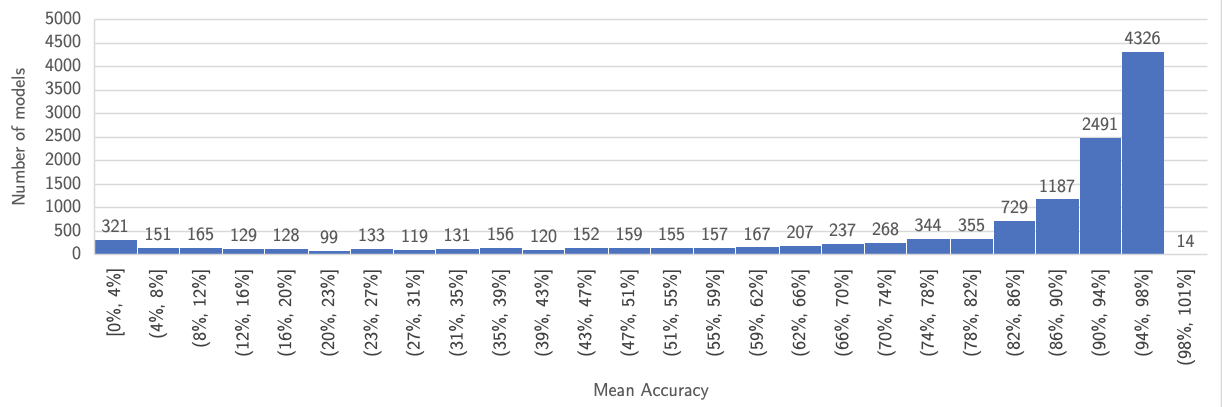
\includegraphics[width=\textwidth]{report/figures/gridsearch_results.png}}
\caption{\label{fig:gridsearch_results}Distribution of the accuracies of the 12,600 combinations of hyperparameters tested with the grid search algorithm.}
\end{figure}

It is interesting to note that over half of these tests result in accuracies range between [90\%-98\%[. This is likely due to the fact that there is very little data to begin with (only 250 entry points), meaning that unless the chosen hyperparameters are really poor performance-wise (e.g. 3 hidden units with momentum 0.1 and tolerance 1, resulting in a mean accuracy of 5.5\%), the neural network will always train to an acceptable level. The lack of data is also a convincing argument to avoid finding optimal general parameters through validation.

\subsubsection{Error Loss and Confusion Matrices}
\label{sec:eval-errorloss-cm}

Four optimal combinations of hyperparameters have been chosen for comparison, along with one set of poor hyperparameters to point out differences. These can be found in Table \ref{tab:nn_hyperparam_eval}.

\begin{table}[h]
\centering
\begin{tabular}{|c|c|c|c|c|c|c|c|}
\hline
\textbf{Activation}             & \textbf{\begin{tabular}[c]{@{}c@{}}Hidden\\ Neurons\end{tabular}} & \textbf{$\alpha$}          & \textbf{$\beta$}           & \textbf{\begin{tabular}[c]{@{}c@{}}N Iter \\ \\ No Change\end{tabular}} & \textbf{Solver}             & \textbf{Tol}                  & \textbf{\begin{tabular}[c]{@{}c@{}}Mean \\ \\ Accuracy\end{tabular}} \\ \hline
{\color[HTML]{036400} logistic} & {\color[HTML]{036400} (15,)}                                      & {\color[HTML]{036400} 0.6} & {\color[HTML]{036400} 0.9} & {\color[HTML]{036400} 1000}                                             & {\color[HTML]{036400} adam} & {\color[HTML]{036400} 0.0001} & {\color[HTML]{036400} 98.5\%}                                        \\ \hline
{\color[HTML]{009901} tanh}     & {\color[HTML]{009901} (5,)}                                       & {\color[HTML]{009901} 0.8} & {\color[HTML]{009901} 0.1} & {\color[HTML]{009901} 100}                                              & {\color[HTML]{009901} sgd}  & {\color[HTML]{009901} 0.0001} & {\color[HTML]{009901} 98.0\%}                                        \\ \hline
{\color[HTML]{009901} logistic} & {\color[HTML]{009901} (9,)}                                       & {\color[HTML]{009901} 0.2} & {\color[HTML]{009901} 0.9} & {\color[HTML]{009901} 1000}                                             & {\color[HTML]{009901} adam} & {\color[HTML]{009901} 0.1}    & {\color[HTML]{009901} 98.0\%}                                        \\ \hline
{\color[HTML]{009901} tanh}     & {\color[HTML]{009901} (25,)}                                      & {\color[HTML]{009901} 1}   & {\color[HTML]{009901} 0.1} & {\color[HTML]{009901} 1000}                                             & {\color[HTML]{009901} sgd}  & {\color[HTML]{009901} 0.001}  & {\color[HTML]{009901} 98.0\%}                                        \\ \hline
{\color[HTML]{CB0000} logistic} & {\color[HTML]{CB0000} (3,)}                                       & {\color[HTML]{CB0000} 1}   & {\color[HTML]{CB0000} 0.5} & {\color[HTML]{CB0000} 1000}                                             & {\color[HTML]{CB0000} adam} & {\color[HTML]{CB0000} 0.001}  & {\color[HTML]{CB0000} 38.0\%}                                        \\ \hline
\end{tabular}
\caption{The 5 neural network hyperparameters used for evaluation, including 4 optimal and 1 sub-optimal.}
\label{tab:nn_hyperparam_eval}
\end{table}

Plotting the error function with respect to the number of epochs required to reach the designated tolerance gives interesting insights about the training, as seen in Figure \ref{fig:error-loss-curve}. Indeed, the error loss curves are all similar when using optimal parameters, quickly converging towards the desired error. A notable difference is the effect of a low momentum $\beta=0.1$ on the convergence speed, causing the light blue slope (5 hidden neurons) to reach the desired error more slowly than neural networks with high momentum.

\begin{figure}[h] 
\centerline{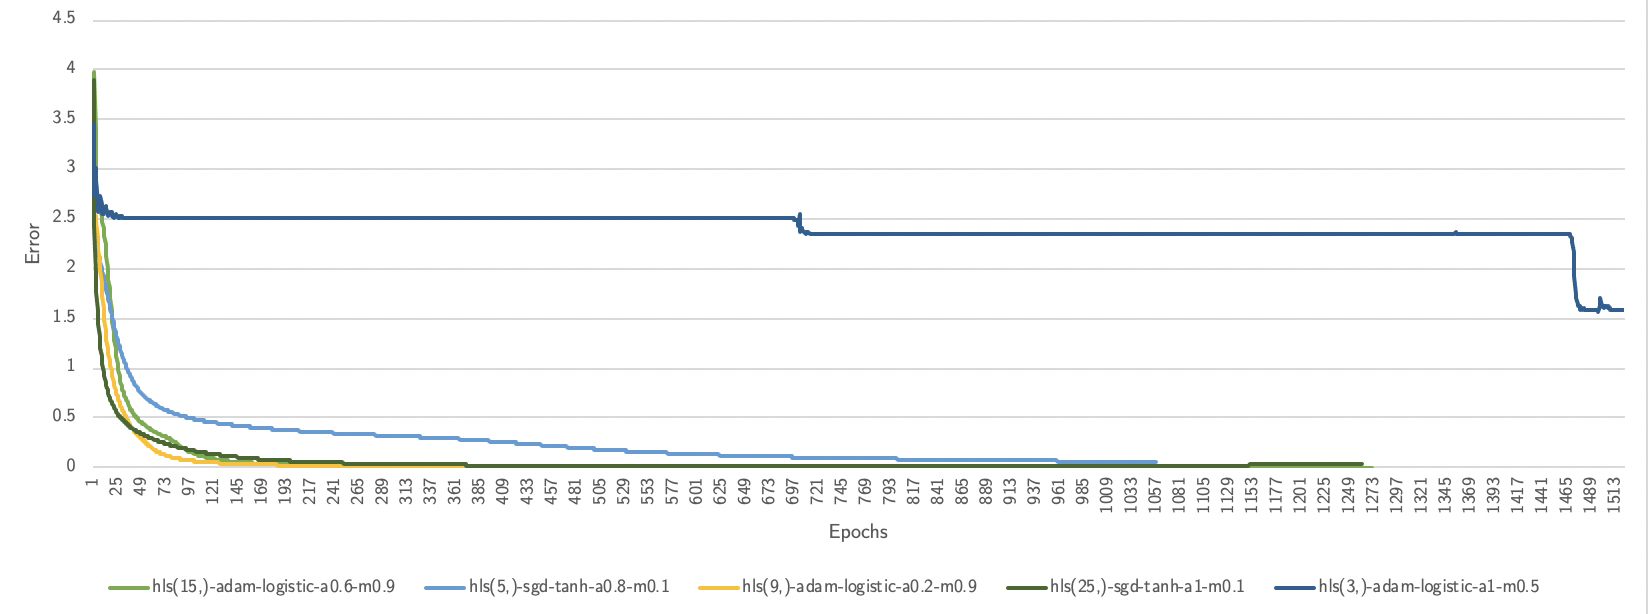
\includegraphics[width=\textwidth]{report/figures/error_loss_curve.png}}
\caption{\label{fig:error-loss-curve}Error loss curves during the training of 5 different combinations of hyperparameters.}
\end{figure}

However, the most notable difference between training with optimal parameters (accuracy $\geqslant$ 98\%) and sub-optimal parameters (accuracy = 38\%) is that the error loss curve is less smooth (small peaks can be seen across the curve before epoch 50) due to the high learning rate and lack of neural units (data is under-fitted). The curve is also characterised by multiple plateaus (straight lines with no improvements) and small ravines (minor increases in error), which would be solved with an increased momentum.\\

Once the training is completed, an aggregated confusion matrix over five runs is calculated and plotted in a heatmap for each neural network. This clearly shows the superior accuracy of neural networks using optimal hyperparameters compared to sub-optimal hyperparameters. The results can be seen in Figure \ref{fig:confusion_matrices}.

\begin{figure}[h] 
\centerline{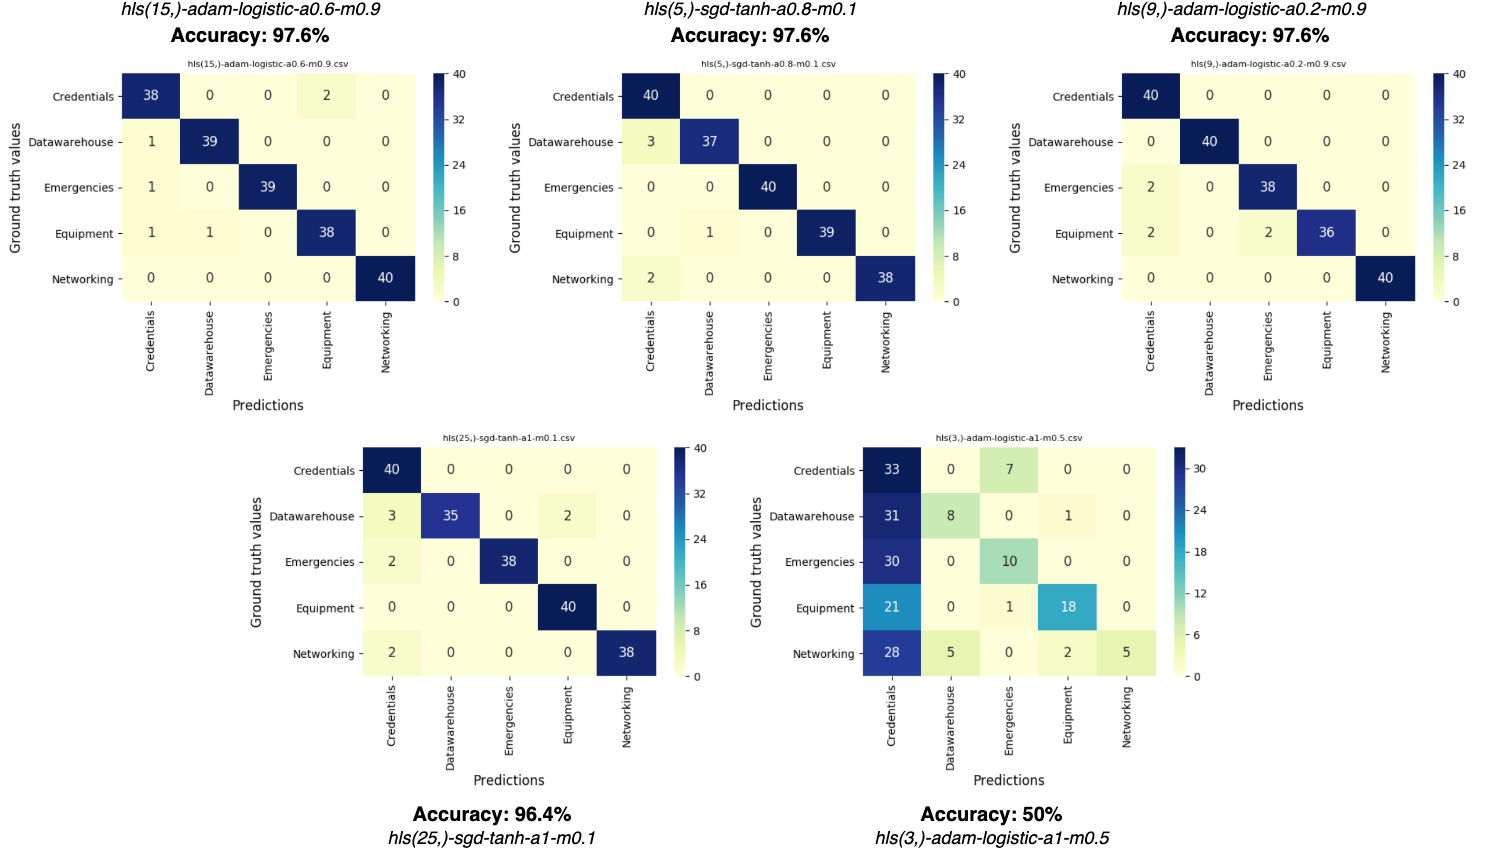
\includegraphics[width=1.1\textwidth]{report/figures/confusion_matrices.png}}
\caption{\label{fig:confusion_matrices}5-run aggregate confusion matrices of the 5 different combinations of hyperparameters.}
\end{figure}

\subsubsection{Ticketing Routing Agent}

The intermediate agent is evaluated by interacting with the CLI-based agent. The full interaction used for this evaluation can be found in Appendix \ref{sec:console-output-example}. It can be seen that when the user creates a new ticket with \textit{``No''} answered to every question, the agent predicts it should go to \textit{Networking}. The user then suggests sending it to \textit{Emergencies} and the neural network is consequently retrained (lines 49 to 53). When submitting a new ticket with the re-trained neural network, the agent immediately predicts that the ticket should go the \textit{Emergencies} after only three questions (line 62), proving that it correctly learned from its mistake.\\

However, this is not always the case, as for cases where tags are similar for different outputs, a single team suggestion is not enough to shift the weights of the neural network for the agent to correctly predict the answer for the next iteration. If a dozen or more users all suggested the same correction to the agent, then the weights would change enough to allow the suggested team to be predicted.\\

\textit{Design, Implementation \& Evaluation Section word count: \underline{XXXX}}

% -------------------------------------- 3 - TEST SUMMARY ------------------------------------------ 
\section{Test Summary}
\label{sec:test-summary}

\subsection{Basic Agent Testing}

The basic agent mainly consists in implementing a neural network using the Scikit library for Python. There is therefore no need to test the functions provided by Scikit.

\subsection{Intermediate Agent Testing}

The intermediate agent's behaviour is tested by ensuring that each prediction (early or not) are correct. This is done by checking that the answers to each question specified in Figure \ref{fig:intermediate_testing} (retrieved from the original \textit{tickets.csv} data file) correspond to the expected output. The green categories indicate a correct prediction. The full interaction between the user and the agent can be found in Appendix \ref{sec:console-output-testing}, with each correct prediction highlighted in yellow.

\begin{figure}[h] 
\centerline{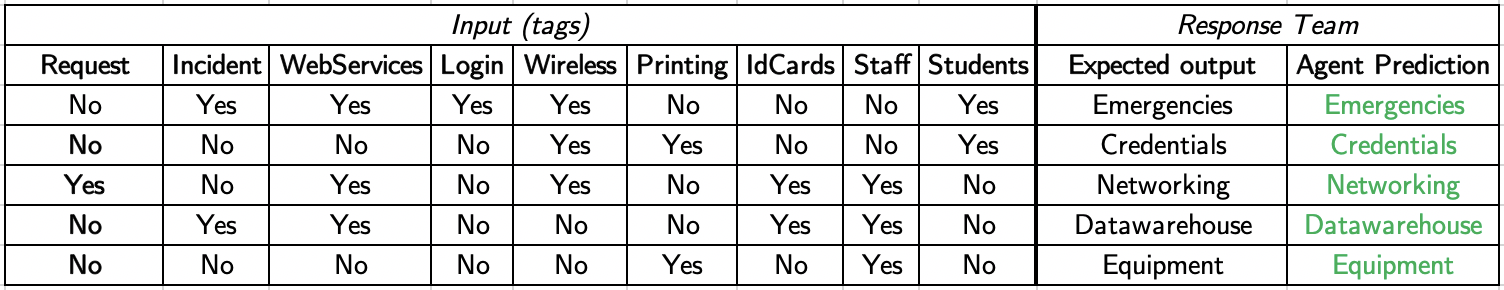
\includegraphics[width=\textwidth]{report/figures/intermediate_testing.png}}
\caption{\label{fig:intermediate_testing}Testing table for the intermediate agent, showing correct predictions for each response team.}
\end{figure}

Regarding the actual functionality of the agent's text-based CLI, edge cases are entered on the command line to show the robustness of the program. The full interaction can be found in Appendix \ref{sec:console-output-edge-cases}. Various inputs are used to answer \textit{``Yes''}/\textit{``No''} questions, such as \textit{y}, \textit{yy}, \textit{YeS}, \textit{YES}, \textit{No}, \textit{NO}, \textit{nn} and \textit{n} (lines 11 to 28). The same is repeated for the response team suggestion: the agent does not let the user input a wrong team, and will ask the question again if wrong input is given (lines 33 to 37). The user can correctly exit the program at any time by typing \textit{``quit''}.


% -------------------------------------- APPENDICES ------------------------------------------ 
\begin{appendices}

\clearpage
\bibliographystyle{plain}
\bibliography{bibliography}

% ------------------------

\clearpage
\section{Project File Structure}
\label{sec:appendix-project-file-structure}

A screenshot of the project’s file structure in the PyCharm IDE to illustrate the organisation of the Python modules and the data used.

\begin{figure}[h] 
\centerline{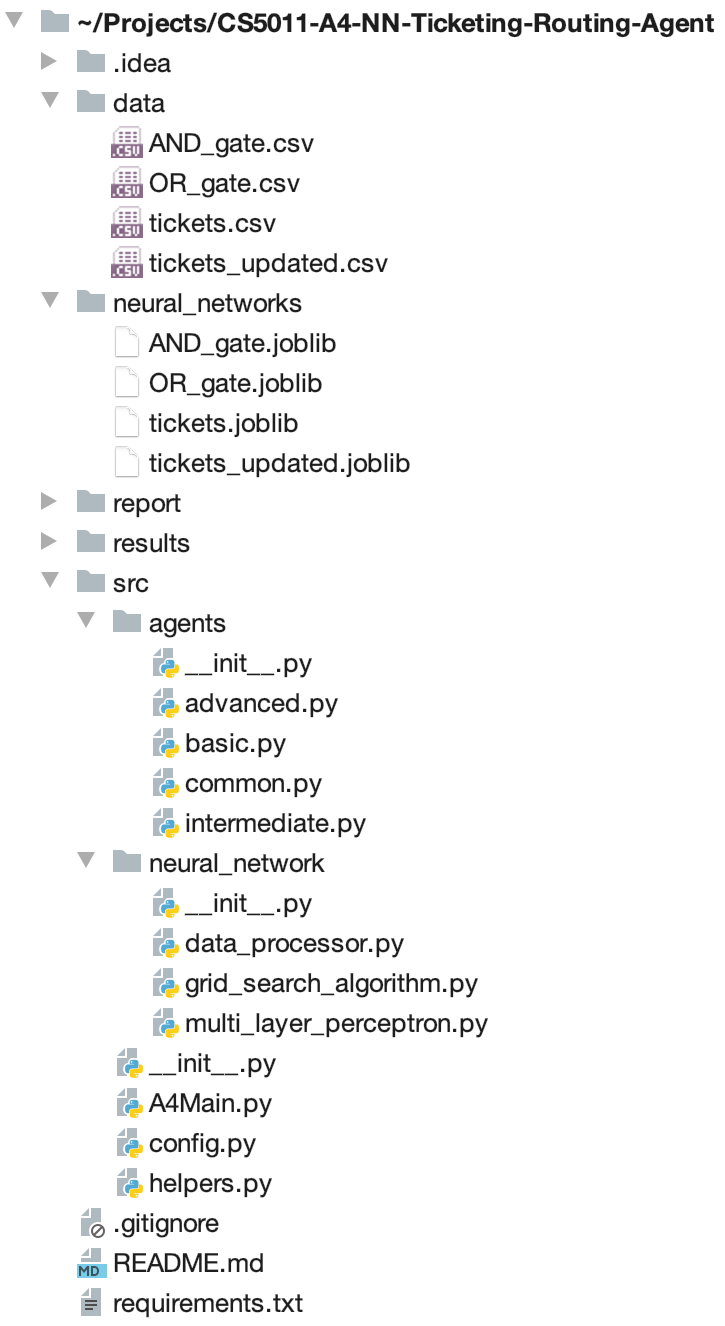
\includegraphics[width=0.55\textwidth]{report/figures/project_structure.png}}
\label{fig:project_structure}
\end{figure}

% ------------------------

\clearpage
\section{Optimal Hyperparameters}
\label{sec:appendix-optimal-hyperparameters}

\begin{landscape}
\begin{table}[]
\begin{tabular}{|c|c|c|c|c|c|c|c|c|}
\hline
\textbf{Activation} & \textbf{\begin{tabular}[c]{@{}c@{}}Hidden \\ \\ Layer \\ \\ Size\end{tabular}} & \textbf{\begin{tabular}[c]{@{}c@{}}Learning \\ \\ Rate\end{tabular}} & \textbf{Momentum} & \textbf{\begin{tabular}[c]{@{}c@{}}N Iter \\ \\ No Change\end{tabular}} & \textbf{Solver} & \textbf{Tolerance} & \textbf{\begin{tabular}[c]{@{}c@{}}Mean \\ \\ Accuracy\end{tabular}} & \textbf{\begin{tabular}[c]{@{}c@{}}Mean \\ \\ Fit Time \\ \\ (seconds)\end{tabular}} \\ \hline
logistic            & (15,)                                                                          & 0.6                                                                  & 0.9               & 1000                                                                    & adam            & 0.0001             & 98.5\%                                                               & 1.61                                                                                 \\ \hline
tanh                & (5,)                                                                           & 0.4                                                                  & 0.7               & 100                                                                     & sgd             & 0.0001             & 98.0\%                                                               & 0.51                                                                                 \\ \hline
tanh                & (5,)                                                                           & 0.8                                                                  & 0.1               & 100                                                                     & sgd             & 0.0001             & 98.0\%                                                               & 0.61                                                                                 \\ \hline
tanh                & (5,)                                                                           & 1                                                                    & 0.3               & 1000                                                                    & sgd             & 1                  & 98.0\%                                                               & 0.77                                                                                 \\ \hline
logistic            & (9,)                                                                           & 0.2                                                                  & 0.9               & 1000                                                                    & adam            & 0.1                & 98.0\%                                                               & 0.78                                                                                 \\ \hline
tanh                & (5,)                                                                           & 0.05                                                                 & 0.9               & 1000                                                                    & adam            & 0.1                & 98.0\%                                                               & 0.80                                                                                 \\ \hline
tanh                & (15,)                                                                          & 0.8                                                                  & 0.7               & 1000                                                                    & sgd             & 0.01               & 98.0\%                                                               & 0.81                                                                                 \\ \hline
tanh                & (5,)                                                                           & 1                                                                    & 0.7               & 1000                                                                    & sgd             & 0.001              & 98.0\%                                                               & 0.86                                                                                 \\ \hline
tanh                & (9,)                                                                           & 0.2                                                                  & 0.3               & 1000                                                                    & adam            & 0.1                & 98.0\%                                                               & 0.92                                                                                 \\ \hline
tanh                & (25,)                                                                          & 0.4                                                                  & 0.9               & 1000                                                                    & sgd             & 1                  & 98.0\%                                                               & 0.93                                                                                 \\ \hline
tanh                & (5,)                                                                           & 0.05                                                                 & 0.9               & 1000                                                                    & sgd             & 0.001              & 98.0\%                                                               & 0.93                                                                                 \\ \hline
logistic            & (25,)                                                                          & 0.4                                                                  & 0.9               & 1000                                                                    & adam            & 0.01               & 98.0\%                                                               & 0.95                                                                                 \\ \hline
tanh                & (25,)                                                                          & 1                                                                    & 0.1               & 1000                                                                    & sgd             & 0.001              & 98.0\%                                                               & 1.12                                                                                 \\ \hline
logistic            & (9,)                                                                           & 0.4                                                                  & 0.3               & 1000                                                                    & sgd             & 0.0001             & 98.0\%                                                               & 1.65                                                                                 \\ \hline
\end{tabular}
\caption{The 14 optimal hyperparameters founds after the grid search algorithm on 12,600 combinations.}
\label{tab:optimal-hyperparameters}
\end{table}
\end{landscape}

% ------------------------

\clearpage
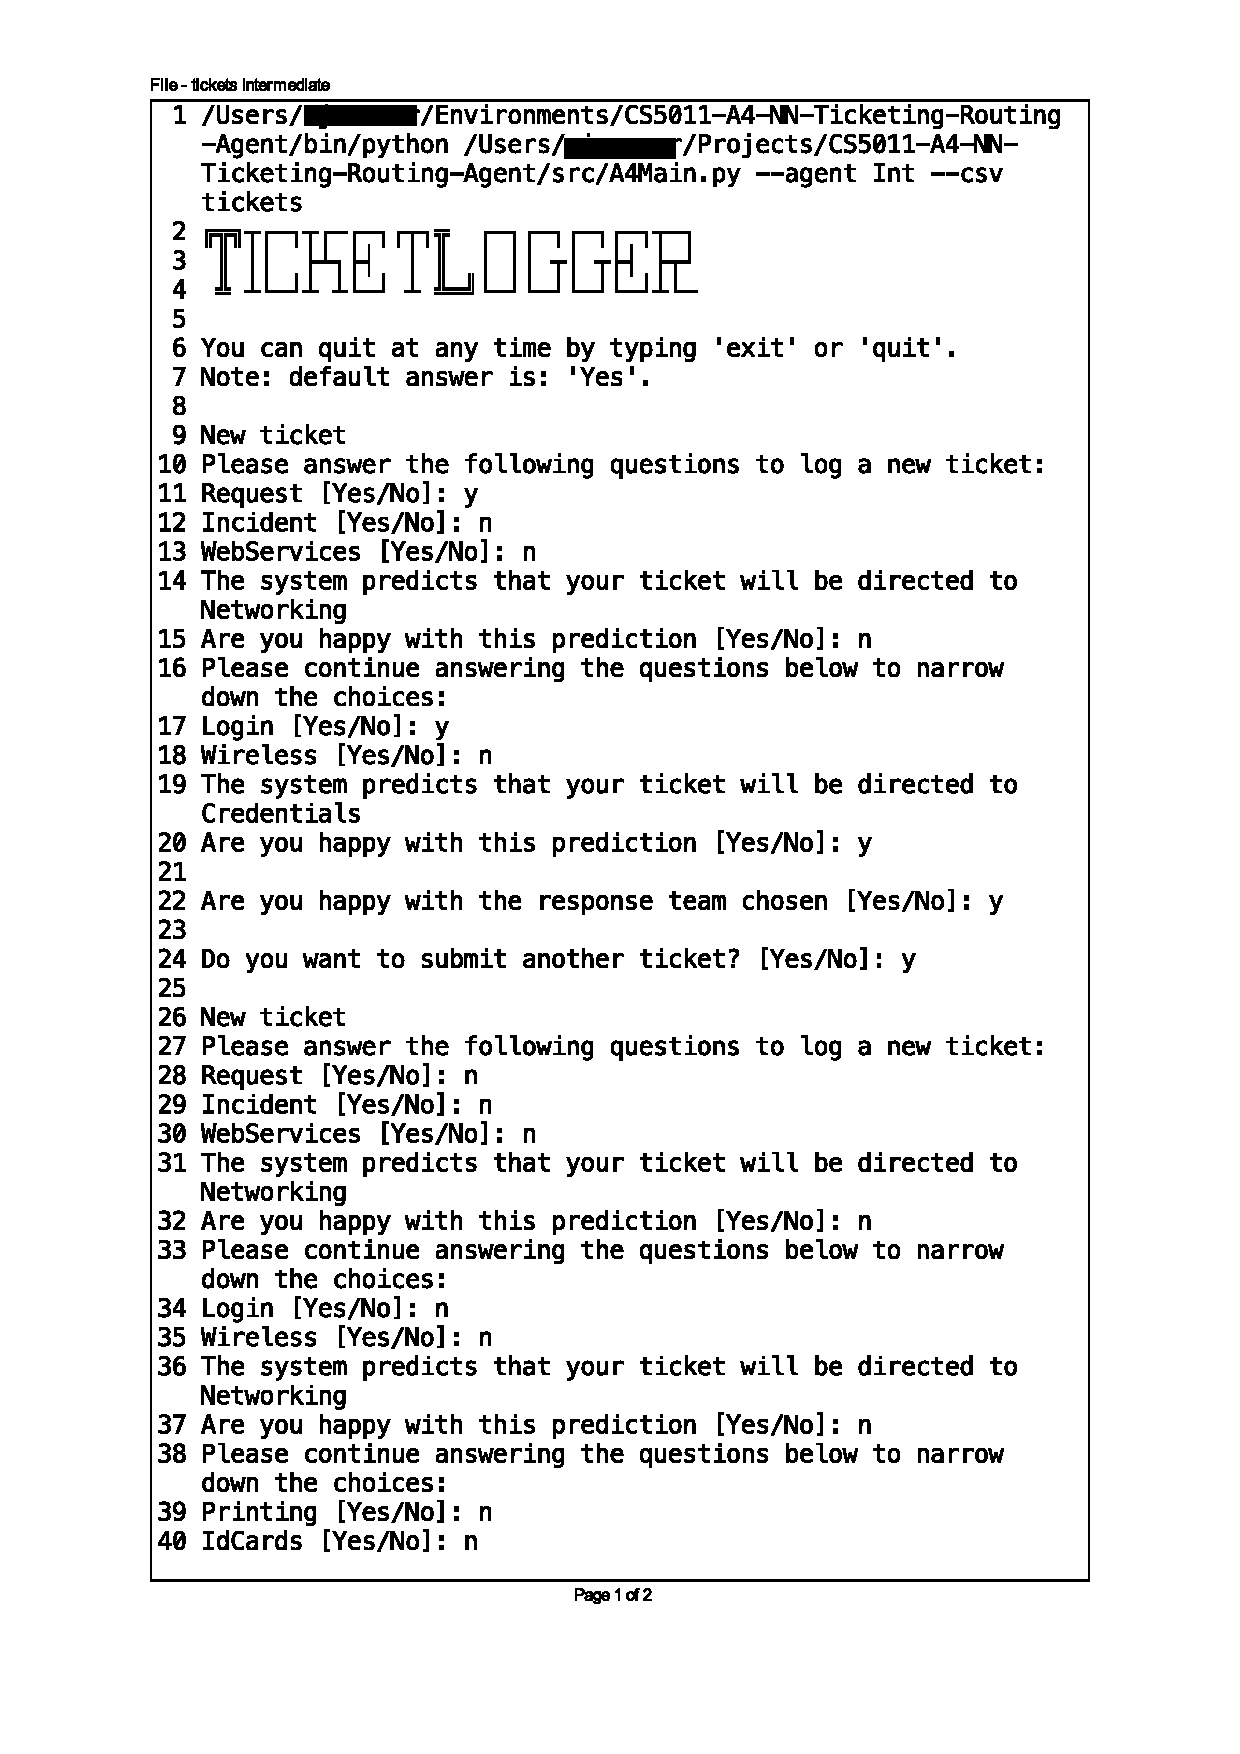
\includepdf[
    pages=1, 
    scale=0.8, 
    pagecommand=\section{Ticketing-Routing Agent Console Output Example}\label{sec:console-output-example}
]{figures/cli-output-evaluation.pdf}
\includepdf[
    pages=2, 
    scale=0.8
]{figures/cli-output-evaluation.pdf}

% ------------------------

\clearpage
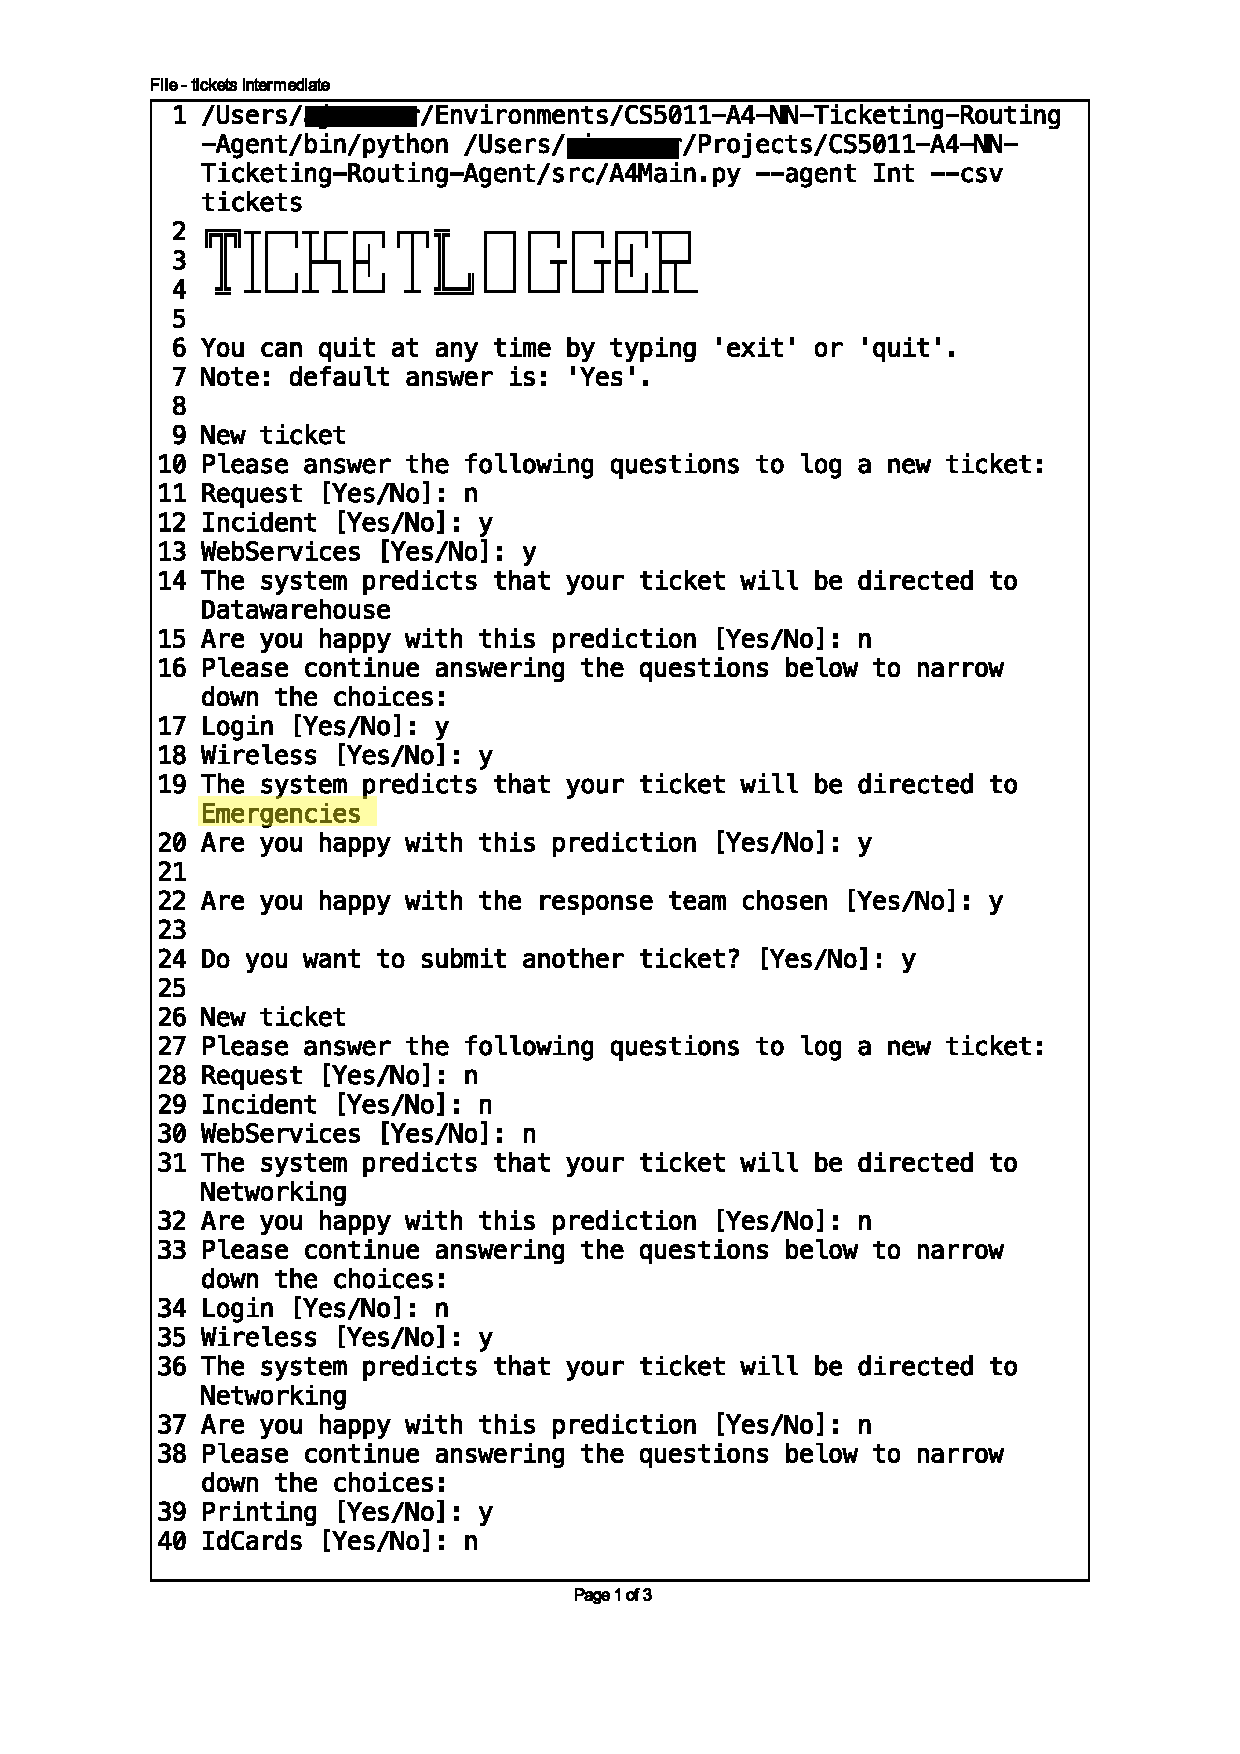
\includepdf[
    pages=1, 
    scale=0.8, 
    pagecommand=\section{Intermediate Agent Prediction Testing}\label{sec:console-output-testing}
]{figures/cli-output-testing.pdf}
\includepdf[
    pages=2, 
    scale=0.8
]{figures/cli-output-testing.pdf}
\includepdf[
    pages=3, 
    scale=0.8
]{figures/cli-output-testing.pdf}

% ------------------------

\clearpage
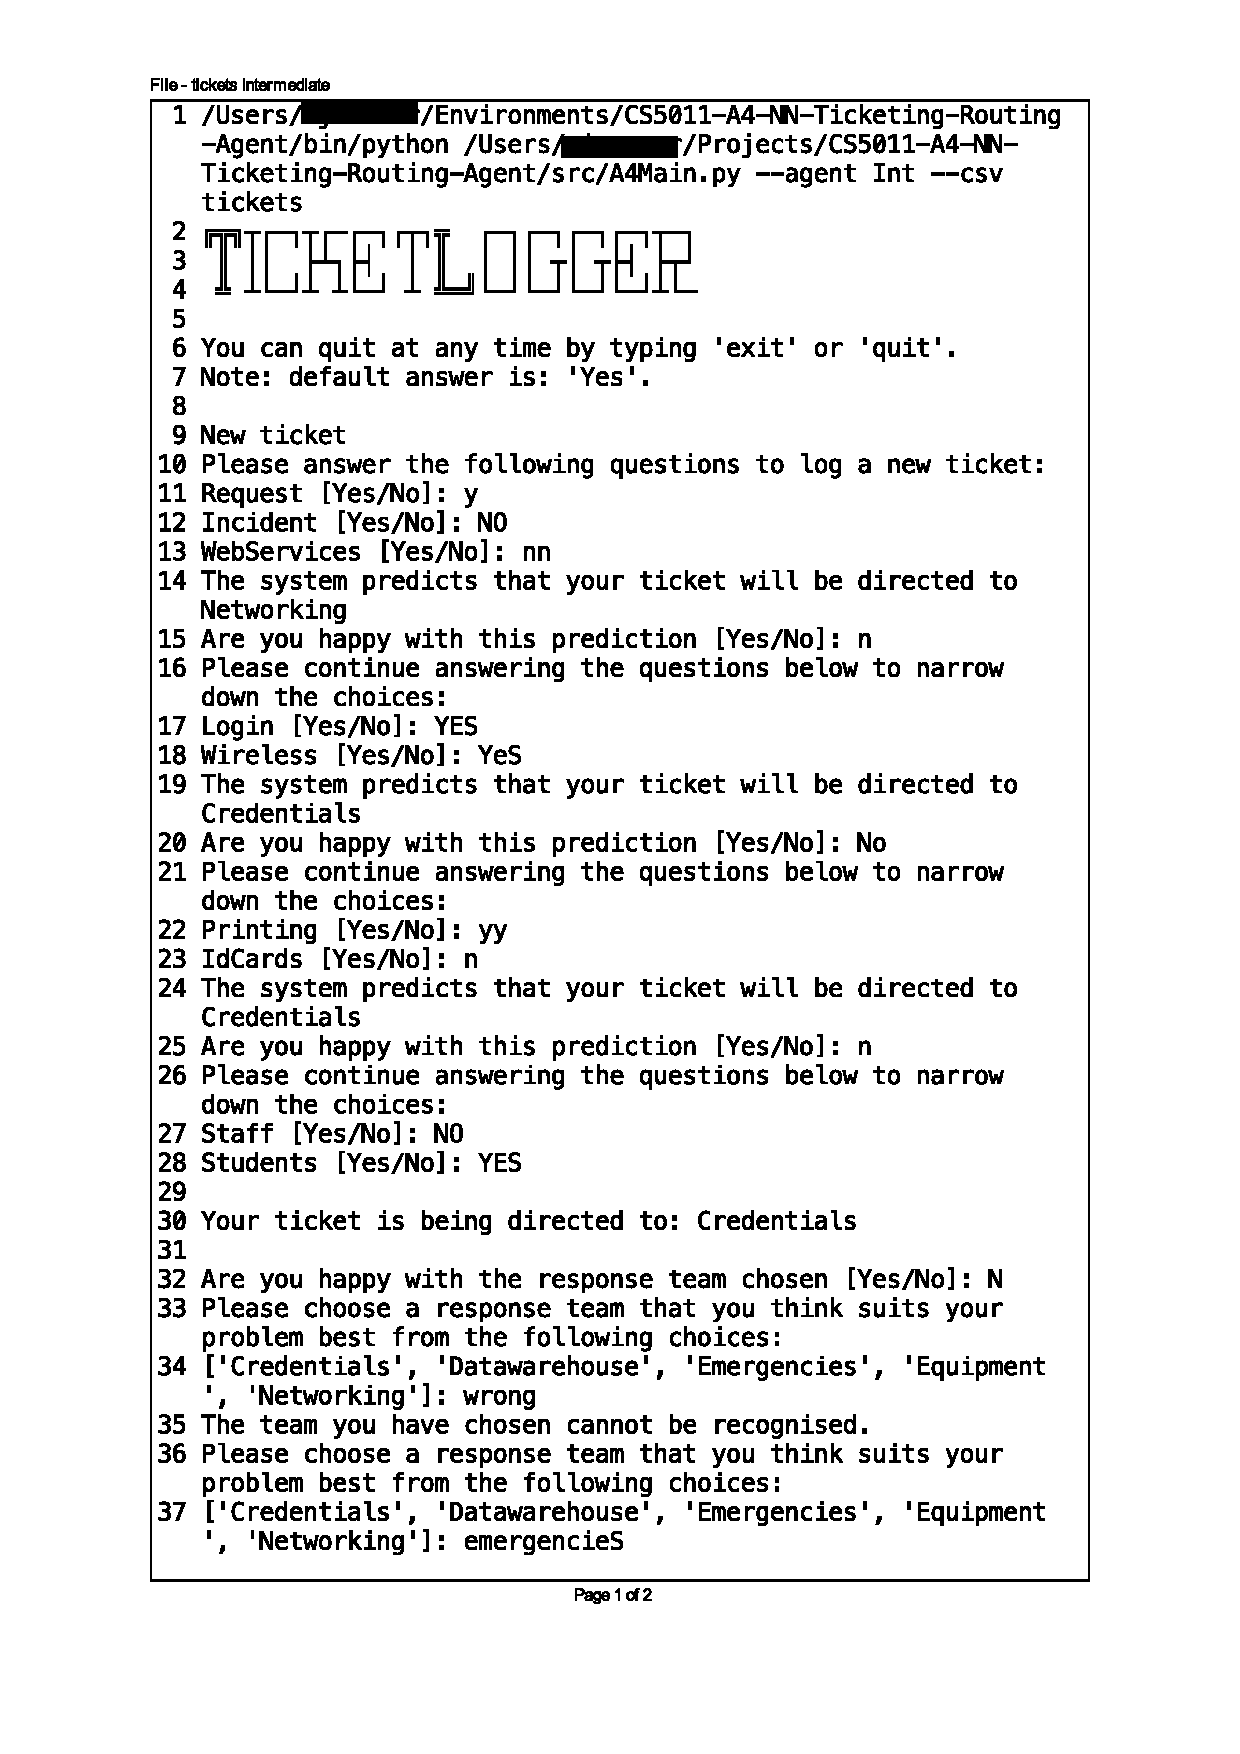
\includepdf[
    pages=1, 
    scale=0.8, 
    pagecommand=\section{Intermediate Agent Text-Based Interface Testing}\label{sec:console-output-edge-cases}
]{figures/cli-output-edge-cases.pdf}
\includepdf[
    pages=2, 
    scale=0.8
]{figures/cli-output-edge-cases.pdf}

% ------------------------

\end{appendices}
\end{document}